\documentclass{article}

\usepackage{nips_like}
\usepackage{config}

\title{PILCO}
\author{
    Xingdong Zuo\thanks{\today} \\
    %\\
    %% \And or \AND
    %% Coauthor \\
    %% Affiliation \\
    %% Address \\
    %% \texttt{email} \\
}

\begin{document}

\maketitle

\section{Key idea}
\begin{itemize}
    \item Reduce sample complexity: prior knowledge (e.g. demonstration) / extracting more information (e.g. learn dynamics)
    \item Model bias in model-based RL: use probabilistic model instead of deterministic
    \item Probabilistic model: GP (sample efficient in low-dim, unscalable) , BNN, ensembles
    \item PILCO: propagate state distribution analytically via GP and incorporate the uncertainty into planning and policy evaluation. 
\end{itemize}

\section{Method}

\begin{algorithm}[H]
    \SetAlgoNoLine
    Randomly initialize the policy $\pi_\theta$ \\
    \For{\textrm{iteration} = 1, 2, \dots}{
    	Execute the system with $\pi_\theta$ and augment the dataset. \\
        Re-train dynamics model. \\
        \For{\textrm{optimization iteration} = 1, \dots, 1000}{
        	Predict system trajectories from $p(X_0)$ to $p(X_T)$. \\
            Evaluate the policy: $J(\theta) = \sum_{t=0}^{T}\gamma^t\Exp{\mathrm{cost}(X_t)}{X}$. \\
            Optimize the policy: $\theta\leftarrow \argmin_{\theta}J(\theta)$
        }
    }
    \caption{PILCO \cite{deisenroth2011pilco}}
    \label{algo:pilco}
\end{algorithm}

\begin{algorithm}[H]
    \SetAlgoNoLine
    Randomly initialize the policy $\pi_\theta$ \\
    \For{\textrm{iteration} = 1, 2, \dots}{
    	Execute the system with $\pi_\theta$ and augment the dataset. \\
        Re-train BNN dynamics model. \\
        \For{\textrm{optimization iteration} = 1, \dots, 1000}{
            Predict system trajectories from $p(X_0)$ to $p(X_T)$. \\
            Sample $K$ particles from initial distribution $x_0^k\sim p(X_0)$ \\
            Sample $K$ set of weights for BNN dynamics model $\{ W^{(k)} \}_{k=1}^{K}$ \\
            \For{t = 1, \dots, T}{
                Obtain output particles $\{ y_{t}^{(k)} \}$ by evaluating $\{ W^{(k)} \}$ and $\{ x_{t}^{(k)} \}$ for all $k = 1, \dots, K$ \\
                Calculate the mean $\mu_t$ and standard deviation $\sigma^t$ of $\{ y_{t}^{(1)}, \dots, y_{t}^{(K)} \}$ \\
                Sample new set of $K$ particles $x_{t+1}^{(k)}\sim\mathcal{N}(\mu_t, \sigma_t^2)$
            }
            Evaluate the policy: $J(\theta) = \sum_{t=0}^{T}\gamma^t\Exp{\mathrm{cost}(X_t)}{X}$. \\
            Optimize the policy: $\theta\leftarrow \argmin_{\theta}J(\theta)$
        }
    }
    \caption{Deep PILCO \cite{gal2016improving}}
    \label{algo:deeppilco}
\end{algorithm}

\begin{figure}[h!]
  \centering
  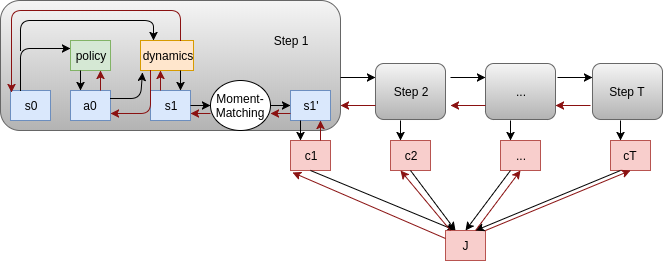
\includegraphics[width=0.9\textwidth]{img/deepilcograph.png}
  \caption{Computational graph of DeepPILCO.}
  \label{fig:deeppilcograph}
\end{figure}

\printbibliography

\end{document}